\appendix

\section{Appendix}

\subsection{Approximation guarantee}\label{app:threshold}
% Note: labels don't work right now because we're not numbering subsections (style file issue)

Let us introduce some notation for the analysis of
Algorithm~\ref{alg:r-domset}. We first partition the vertices of~$D$ according
to whether they were added in line~\ref{algstep:D1} (denoted by~$D_1$) or in
line~\ref{algstep:D2} (denoted by~$D_2$). Let~$v_1,\ldots,v_n$ be the vertex-
order in which they are iterated over in the loop starting at
line~\ref{algstep:order}. We will use the notation~$D_1^i$, $D_2^i$, $d^i$,
and~$c^i$ to represent the states of the respective sets and data structures
during the $i$th iteration of said loop. Let~$\tau :=
\texttt{domThreshold}(r)$ be the chosen threshold (we discuss a good value
for $\tau$ on cDBGs below).

\begin{lemma}
  After the for-loop at line~\ref{algstep:pull} has finished,
  \[
    d^i[v_i] = \begin{cases*}
      \dist_G(v,D^i) & if $\dist_G(v,D^i) \leq r$, and \\
      \infty & otherwise.
    \end{cases*}
  \]
\end{lemma}
\begin{proof}
  The statement trivially holds while~$D^i = \emptyset$, so assume otherwise.
  Let~$u_h \in D^i$ be the vertex closest to~$v_i$ and let~$h < i$
  be the iteration in which~$u_h$ was added to~$D$ (either in
  line~\ref{algstep:D1} or line~\ref{algstep:D2} of that iteration).

  If $d := \dist_G(v_i,u_h) > r$,
  then~$d^i[v_i]$ has not been changed yet and is still set to~$\infty$.
  Otherwise, consider the three possible scenarios promised by the
  distance-property of dtf-augmentations:

  \begin{case}[$v_iu_h \in \dir G_d$]
    Then~$\omega(v_iu_h) = d$ and in iteration~$h$
    the value of~$d^h[v_i]$ is set to the correct value~$d$
    in the loop at line~\ref{algstep:pull}.
    By assumption this distance remains minimal until iteration~$i$
    and hence~$d^i[v_i] = d^h[v_i] = d$.
  \end{case}

  \begin{case}[$u_hv_i \in \dir G_d$]
    Then~$\omega(v_iu_h) = d$ and in iteration~$i$
    the value of~$d^i[v_i]$ is set to the correct value~$d$
    in the loop at line~\ref{algstep:pull}.
  \end{case}

  % The cases env is a bit hacky. Parenthesis don't work well,
  % unless hidden in a macro.
  \def\ww#1{\omega(#1)}
  \begin{case}[$xu_h,xv_i \in \dir G_d$  with~$\ww{xu_h} + \ww{xv_i} = d$]\mbox{}\\
    During iteration~$h$ the value of~$d^h[x]$ is set to~$\ww{xu_h}$
    in the loop at line~\ref{algstep:pull} and subsequently retrieved
    in iteration~$i$ when $d^i[v_i]$ is set to
    \[
      d^i[x] + \ww{xu_h} = \ww{xu_h} + \ww{xv_i} = d.
    \]
    \vspace*{-1.5em}
  \end{case}
  \noindent
  We conclude that after the execution of the loop at line~\ref{algstep:pull}.
  $d^i[v_i]$ is set to~$\infty$ if~$v_i$ is not dominated by~$D_i$ and is
  otherwise set to~$\dist_G(v_i,D^i)$, as claimed.
\end{proof}

\noindent
As an immediate consequence, we see the conditional statement at the end of
the loop at line~\ref{algstep:pull} accurately determines whether $v_i$ is
dominated by~$D_i$ or not. Accordingly, lines~\ref{algstep:D2}
of the loop are only executed if~$v_i$ is \emph{not} dominated by~$D^i$.
Another consequence is that all vertices in~$D_1$ have large distance to
each other:

\begin{corollary}
  The set~$D_1$ is $(r+1)$-scattered in~$G$.
\end{corollary}

\noindent
We need one more important property of the algorithm in order to derive
the approximation factor.

\begin{lemma}\label{lemma:D1-intersection}
  For every~$w \in G$ it holds that~$|D_1 \cap N^-_r(w)| \leq \tau+1$.
\end{lemma}
\begin{proof}
  Assume towards a contradiction that~$\tau+2$ such vertices
  $v_{i_1},\ldots,v_{i_\tau+2}$, $i_1 < i_2 < \ldots < i_{\tau+2}$ exist in~$D_1
  \cap N^-_r(w)$. Since every such vertex~$v_i$, $i \in \{i_1,\ldots
  i_{\tau+2}\}$, was added to~$D$ in part~\MARK{2}, part~\MARK{3} of the
  algorithm was executed during iteration~$i$ as well. Thus~$c[w]$ was
  increased in each iteration~$i$ and during iteration~$i_{\tau+1}$ we have that
  $c[w] \geq \tau + 1$ after the increment of~$c[w]$. Therefore part~\MARK{4}
  must have been executed for~$w$, including~$w$ into~$D$. Hence~$w \in D^s$
  for~$s > i_{\tau+1}$ and in particular $w \in D^{i_{\tau+2}}$. But then
  $v_{i_{\tau+2}}$ was dominated by~$w$ at the beginning of iteration~$i_{\tau+2}$
  since we assumed that~$\omega(rv_{i_{\tau+2}}) \leq r$, thus~$v_{i_{\tau+2}}$
  would not have been included in~$D$ at step~\MARK{2}. This contradicts our
  assumption of $v_{i_{\tau+2}} \in D_1$ so the claim must hold.
\end{proof}


\begin{lemma}
  There exists a subset~$A \subseteq D_1$ such that~$A$ is
  $(2r+1)$-scattered in~$G$ and
  \[
  	|A| \geq \frac{|D|}{2(\tau+2)\maxindeg(\dir G_{2r}))\maxindeg(\dir G_r)}.
  \]
\end{lemma}
\begin{proof}
  We construct an auxiliary graph~$H$ with vertices~$D_1$ by
  adding arcs~$v_iv_j$ for $v_i,v_j \in D_1$ with $i < j$
  whenever~$\dist_G(v_i,v_j) \leq 2r$.
  Let~$\dir G_{2r}$ be a $2r$th dtf-augmentation of~$G$ and
  let us create a digraph~$\dir H$ by orienting
  every edge~$uv \in H$ as follows:
  \begin{enumerate}
    \item If of~$uv,vu \in \dir G_{2r}$,
          then orient~$uv$ in~$\dir H$ according to the corresponding
          arc in $\dir G_{2r}$ (if both arcs exists choose an arbitrary
          orientation),
    \item otherwise there exists~$w \in N^-_{2r}(u) \cap N^-_{2r}(v)$
          with~$\omega_{2r}(u) + \omega_{2r}(v) = \dist_G(u,v) \leq 2r$. Orient the edge~$uv$ towards that vertex~$x \in \{u,v\}$
          for which~$\omega_{2r}(x)$ is larger.
  \end{enumerate}
  We now argue that~$\maxindeg(\dir H)$ is small. Consider any vertex $v \in
  \dir H$. Every in-arc $uv \in \dir H$ either is of type~1, of which we have
  at most~$\maxindeg(\dir G_{2r})$, or of type~2. Consider a group of in-
  arcs~$u_iv$, $1 \leq i \leq \ell$ of type~2 that are all present because of
  a common vertex~$w$. Since~$w \in N^-_{2r}(u)$, we have at
  most~$\maxindeg(\dir G_{2r})$ such groups. By construction,
  $\omega_{2r}(wu_i) \leq \omega_{2r}(wv)$ and since both weights sum to less
  than~$2r$, this means that~$\omega_{2r}(wu_i) \leq r$.
  Lemma~\ref{lemma:D1-intersection} now tells us that~$\ell \leq \tau + 1$.
  Therefore~$v$ has at most~$(\tau+1) \maxindeg(\dir G_{2r})$ in-arcs of type~2 and we conclude that
  \[
    \maxindeg(\dir H) \leq \maxindeg(\dir G_{2r}) + (\tau+1)\maxindeg(\dir G_{2r}) = (\tau+2)\maxindeg(\dir G_{2r}).
  \]
  This finally implies that~$H$ is $2(\tau+2)\maxindeg(\dir G_{2r})$-degenerate and therefore contains an independent set~$A \subseteq V(H)$
  of size at least~$|A| \geq |H| / (2(\tau+2)\maxindeg(\dir G_{2r}))$.
  Taken together with the fact that~$|H| = |D_1| \geq |D| / \maxindeg(\dir G_r)$
  (every vertex added to~$D_1$ will cause at most~$\maxindeg(\dir G_r)$ many
  vertices to be added to~$D_2$ in the loop at line~\ref{algstep:pushloop}
  and~$D = D_1 \cup D_2$), we find that
  \[
  	|A| \geq \frac{|D|}{2(\tau+2)\maxindeg(\dir G_{2r}))\maxindeg(\dir G_r)}
  \]
  By construction of~$H$ we conclude that~$A$ is $(2r+1)$-scattered
  in~$G$ of the claimed sized.
\end{proof}

\noindent
Since a $(2r+1)$-scattered set provides a lower bound for an~$r$-dominating set, we conclude that Algorithm~\ref{alg:r-domset}
computes a $2(\tau+2)\maxindeg(\dir G_{2r})\maxindeg(\dir G_r)$-approximation of an
optimal $r$-dominating set, which is a constant-factor approximation in graphs
of bounded expansion.

In practice one could, depending on the value of $\maxindeg(\dir G_r)$
and $\maxindeg(\dir G_{2r})$, compute the optimal value for~$\tau$. However, this
would necessitate the computation of $2r$ augmentation, the expensive step we
want to avoid. Alternatively, we can choose a `good enough' value for $\tau$
that still guarantees a constant-factor approximation while being easy to
determine in practice. In the context of cDBGs, we found that
$\tau := (2r)^2$ yields reliably good results.

\subsection{Computational Runtimes}
\label{subsec:runtimes}

See ``Benchmarking'' in Materials and Methods for benchmarking methods.

The \podarv data set was retrieved from the NCBI SRA using accession
SRR606249.  The full build and indexing of the 103 million
error-trimmed reads (10.3 Gbp in total) took approximately 23 minutes
and required 12.8 GB of RAM. Loading the indices for search required
4.3 GB of RAM and a search with a 3 Mbp genome took approximately 32
seconds.

The \hu data set was retrieved from the NCBI SRA using accession
SRR1976948. The full build and indexing of the 34 million
error-trimmed reads (8.5 Gbp in total) required approximately 217
minutes and required 24.4 GB of RAM. Loading the indices for search
required 18 GB of RAM and a search with a 3 Mbp genome took
approximately 80 seconds.

For data set complexity (number of k-mers, number of cDBG nodes) please see
Table~\ref{tab:data}.

\subsection{Query genome accession numbers for {\em Proteiniclasticum} search}
\label{subsec:query_accessions}

See Table~\ref{tab:query_accessions}.

\begin{table}[b]
  \begin{tabular}{l l c c }
    \toprule
    Name & NCBI accession \\
    \midrule
    \hline
    P. ruminis CGMCC & GCA\_900099635.1 \\
    P. ruminis DSM & GCA\_000701905.1 \\
    P. ruminis ML2 & GCA\_900115135.1 \\
    \hline
    \bottomrule
  \end{tabular}
  \caption{Accession numbers for genomes used in {\em Proteiniclasticum} neighborhood query.}
  \label{tab:query_accessions}
\end{table}

\subsection{Amino Acid Identity results for {\em Proteiniclasticum}}
\label{subsec:aai}

See Table~\ref{tab:aai}.

\begin{table}
  \begin{tabular}{l l c c }
    \toprule
    Genome A & Genome B & Orthologous Genes & Mean AAI \\
    \midrule
    {\em P. ruminis ML2} & {\em P. ruminis shakya} & 2546 & 95.74 \\
    {\em P. ruminis DSM} & {\em P. ruminis shakya}  & 2391 & 93.47 \\
    \hline
    \bottomrule
  \end{tabular}
  \caption{CompareM results for {\em Proteiniclasticum} genomes. {\em P. ruminis shakya} is the result of assembling the reads extracted from \podarv with the neighborhood search.}
  \label{tab:aai}
\end{table}

\subsection{Genome bin completeness improvements for \hu}
\label{subsec:checkm}

See Table~\ref{tab:completeness}.

\begin{table*}
  \parbox[t][][t]{.55\linewidth}{%
  \begin{tabular}{@{}l c c c@{}}
    \toprule
    Bin name & Bin completeness & MEGAHIT ($\Delta$) & \plass ($\Delta$) \\
    \midrule
    % generated from notebook 'figures/fig-hu_strain.ipynb'
    WS6 bacterium 36\_33 & 31.5\% & 51.4\% (19.9) & 46.1\% (14.6) \\
P. bacterium 34\_609 & 34.0\% & 42.4\% (8.4) & 55.0\% (20.9) \\
P. bacterium 33\_209 & 47.9\% & 51.5\% (3.6) & 55.7\% (7.8) \\
M. bacterium 39\_7 & 50.1\% & 50.9\% (0.9) & 66.5\% (16.5) \\
P. acetatigenes isolate 50\_10 & 56.7\% & 60.1\% (3.4) & 60.5\% (3.8) \\
WS6 bacterium 34\_10 & 61.9\% & 67.3\% (5.5) & 66.2\% (4.3) \\
M. infera isolate 46\_47 & 63.8\% & 67.5\% (3.8) & 66.8\% (3.0) \\
A. bacterium 34\_128 & 64.4\% & 75.0\% (10.6) & 68.1\% (3.7) \\
A. thermophila isolate 46\_16 & 67.2\% & 78.3\% (11.1) & 76.6\% (9.4) \\
A. bacterium 49\_20 & 69.5\% & 72.3\% (2.7) & 72.4\% (2.9) \\
M. marisnigri isolate 62\_101 & 72.1\% & 80.8\% (8.6) & 85.7\% (13.6) \\
M. bacterium 46\_47 & 72.9\% & 81.0\% (8.1) & 81.0\% (8.1) \\
B. bacterium & 80.0\% & 79.5\% (-0.5) & 83.7\% (3.7) \\
Methanocalculus sp. 52\_23 & 82.7\% & 87.4\% (4.7) & 91.7\% (9.0) \\
Desulfotomaculum sp. 46\_80 & 83.5\% & 93.1\% (9.6) & 95.8\% (12.3) \\
S. bacterium 57\_84 & 90.8\% & 92.0\% (1.2) & 90.8\% (0.0) \\
S. bacterium 53\_16 & 91.5\% & 94.8\% (3.3) & 94.8\% (3.3) \\
Desulfotomaculum sp. 46\_296 & 91.5\% & 94.0\% (2.4) & 100.0\% (8.5) \\
A. bacterium 66\_15 & 94.2\% & 95.3\% (1.1) & 98.1\% (4.0) \\
C. bacterium 38\_11 & 94.4\% & 96.2\% (1.7) & 96.2\% (1.8) \\
TA06 bacterium 32\_111 & 94.5\% & 94.5\% (0.0) & 96.4\% (1.8) \\
Methanobacterium sp. 42\_16 & 97.6\% & 98.4\% (0.8) & 97.7\% (0.1) \\
M. harundinacea isolate 57\_489 & 100.0\% & 100.0\% (0.0) & 95.8\% (-4.2) \\

 \\
    \bottomrule
  \end{tabular}
  \caption{\label{tab:completeness}%
  Bin and neighborhood completeness, as estimated by CheckM. ``Bin completeness''
  is the result of running CheckM on the genome sequence from GenBank; MEGAHIT
   is the result of running CheckM on the MEGAHIT nucleotide assembly of the
   neighborhood reads; \plass is the result of running CheckM on the \plass
   amino acid assembly of the neighborhood reads. $\Delta$ is the difference
   between the column and the bin completeness.}
  }%
  \hfill
  \parbox[t][][t]{.4\linewidth}{
  \begin{tabular}{@{}l l c c @{}}
    \toprule
    Species & gyrA (bin) & gyrA (\plass) \\
    \midrule
    % generated from notebook 'tables/plass-genes/distinct_positions.ipynb'
    Methanobacterium sp. 42\_16 & 0 & 0 \\
    P. bacterium 34\_609 & 0 & 0 \\
    Desulfotomaculum sp. 46\_80 & 0 & 0 \\
    S. bacterium 57\_84 & 0 & 0 \\
    B. bacterium & 0 & 1 \\
    P. acetatigenes isolate 50\_10 & 0 & 2 \\
    WS6 bacterium 34\_10 & 0 & 2 \\
    M. marisnigri isolate 62\_101 & 0 & 2 \\
    C. bacterium 38\_11 & 1 & 1 \\
    M. infera isolate 46\_47 & 1 & 1 \\
    S. bacterium 53\_16 & 1 & 1 \\
    M. bacterium 46\_47 & 1 & 1 \\
    TA06 bacterium 32\_111 & 1 & 1 \\
    P. bacterium 33\_209 & 1 & 1 \\
    A. bacterium 66\_15 & 1 & 1 \\
    Methanocalculus sp. 52\_23 & 1 & 2 \\
    WS6 bacterium 36\_33 & 1 & 2 \\
    A. bacterium 34\_128 & 1 & 2 \\
    A. thermophila isolate 46\_16 & 1 & 2 \\
    M. harundinacea isolate 57\_489 & 1 & 2 \\
    M. bacterium 39\_7 & 2 & 0 \\
    Desulfotomaculum sp. 46\_296 & 2 & 2 \\
    A. bacterium 49\_20 & 2 & 3 \\
    \bottomrule
  \end{tabular}
  \caption{  \label{tab:gyrAcounts}%
   Bin and neighborhood gyrA protein content. gyrA count for each bin is the number
    of gyrA amino acid sequences that are part of the original bin. gyrA count by \plass is
    the minimum number of gyrA amino acid sequences supported by at least one
    position with at least 10 copies of each variant, e.g. ``3'' indicates that
    there is at least one position in the multiple sequence alignment of gyrA
    sequences for that neighborhood that has 3 distinct variants in 10 distinct
    sequences.}
  }
\end{table*}

\subsection{K-mer inclusion of reads by MEGAHIT assemblies}
\label{subsec:inclusion}

See Table~\ref{tab:kmer_inclusion}. We estimated the number of k-mers in each
query neighborhood that were contained in the MEGAHIT assembly of that query
neighborhood. We used sourmash {\tt compute} to calculate signatures with k-size of
31 and a scaled value of 2000. We then used sourmash {\tt compare} to estimate
containment in MEGAHIT assemblies. The query neighborhood with the smallest 
containment, \emph{M. harundinacea} isolate \emph{57\_489}, had the largest query
neighborhood, while the query neighborhood with the largest containment,
\emph{M. bacterium 39\_7}, had the smallest query neighborhood.  

\begin{table}
  \begin{tabular}{l c}
    \toprule
    Species & MEGAHIT assembly containment \\
    \midrule
    % generated from notebook 'figures/megahit-assembly-inclusion.ipynb'
    M. harundinacea isolate 57\_489 & 4.2\% & 97.8\% \\
Desulfotomaculum sp. 46\_296 & 12.7\% & 97.7\% \\
M. marisnigri isolate 62\_101 & 13.6\% & 97.2\% \\
S. bacterium 57\_84 & 19.4\% & 97.9\% \\
P. bacterium 34\_609 & 19.7\% & 97.9\% \\
A. bacterium 66\_15 & 20.5\% & 96.9\% \\
Desulfotomaculum sp. 46\_80 & 24.1\% & 97.6\% \\
P. bacterium 33\_209 & 26.3\% & 97.6\% \\
S. bacterium 53\_16 & 30.9\% & 98.1\% \\
A. bacterium 49\_20 & 31.9\% & 96.9\% \\
Methanocalculus sp. 52\_23 & 33.4\% & 97.6\% \\
M. bacterium 46\_47 & 36.6\% & 98.4\% \\
P. acetatigenes isolate 50\_10 & 36.6\% & 97.1\% \\
A. bacterium 34\_128 & 36.8\% & 93.4\% \\
M. infera isolate 46\_47 & 38.0\% & 98.3\% \\
Methanobacterium sp. 42\_16 & 38.0\% & 95.2\% \\
A. thermophila isolate 46\_16 & 38.6\% & 95.9\% \\
TA06 bacterium 32\_111 & 44.1\% & 98.8\% \\
C. bacterium 38\_11 & 44.4\% & 96.0\% \\
WS6 bacterium 34\_10 & 53.2\% & 96.1\% \\
WS6 bacterium 36\_33 & 53.8\% & 98.2\% \\
B. bacterium & 54.2\% & 94.9\% \\
M. bacterium 39\_7 & 55.7\% & 95.6\% \\

%    M. bacterium 39\_7 & 0 & 0 \\
P. acetatigenes isolate 50\_10 & 0 & 0 \\
WS6 bacterium 34\_10 & 0 & 0 \\
Methanobacterium sp. 42\_16 & 0 & 0 \\
Methanocalculus sp. 52\_23 & 0 & 0 \\
WS6 bacterium 36\_33 & 0 & 0 \\
M. marisnigri isolate 62\_101 & 0 & 0 \\
B. bacterium & 0 & 0 \\
P. bacterium 33\_209 & 0 & 0 \\
M. harundinacea isolate 57\_489 & 0 & 0 \\
M. infera isolate 46\_47 & 0 & 1 \\
C. bacterium 38\_11 & 1 & 1 \\
A. bacterium 49\_20 & 1 & 1 \\
P. bacterium 34\_609 & 1 & 1 \\
S. bacterium 57\_84 & 1 & 1 \\
S. bacterium 53\_16 & 1 & 1 \\
A. bacterium 34\_128 & 1 & 1 \\
M. bacterium 46\_47 & 1 & 1 \\
TA06 bacterium 32\_111 & 1 & 1 \\
A. bacterium 66\_15 & 1 & 1 \\
A. thermophila isolate 46\_16 & 1 & 1 \\
Desulfotomaculum sp. 46\_80 & 1 & 2 \\
Desulfotomaculum sp. 46\_296 & 1 & 2 \\

    \bottomrule
  \end{tabular}
  \caption{Containment of neighborhood k-mer content in MEGAHIT nucleotide assemblies.}
  \label{tab:kmer_inclusion}
\end{table}

\subsection{gyrA alignment}
\label{subsec:gyrAalign}

See Figure~\ref{fig:gyrAalign}. The MDS plot in the left panel of figure 4 shows
distinct gyrA sequences identified in the Plass assemblies using HMMER. To visualize
the sequences within these clusters and in other query neighborhoods, we 
constructed a multiple sequence alignment. However, because many
sequences assembled by Plass were fragmented (see Results: Some query neighborhoods
contain substantial strain variation), we first clustered the sequences at 95\% 
similarity using CD-HIT. We then aligned the centroid sequences using MAFFT with 
default settings. To produce the multiple sequence alignment visualization, we 
calculated an unrooted neighbor joining tree using the MAFFT alignment. Then we used
the function {\tt msaplot} in the R package ggtree to plot the alignment.  

\begin{figure*}
 \centering
 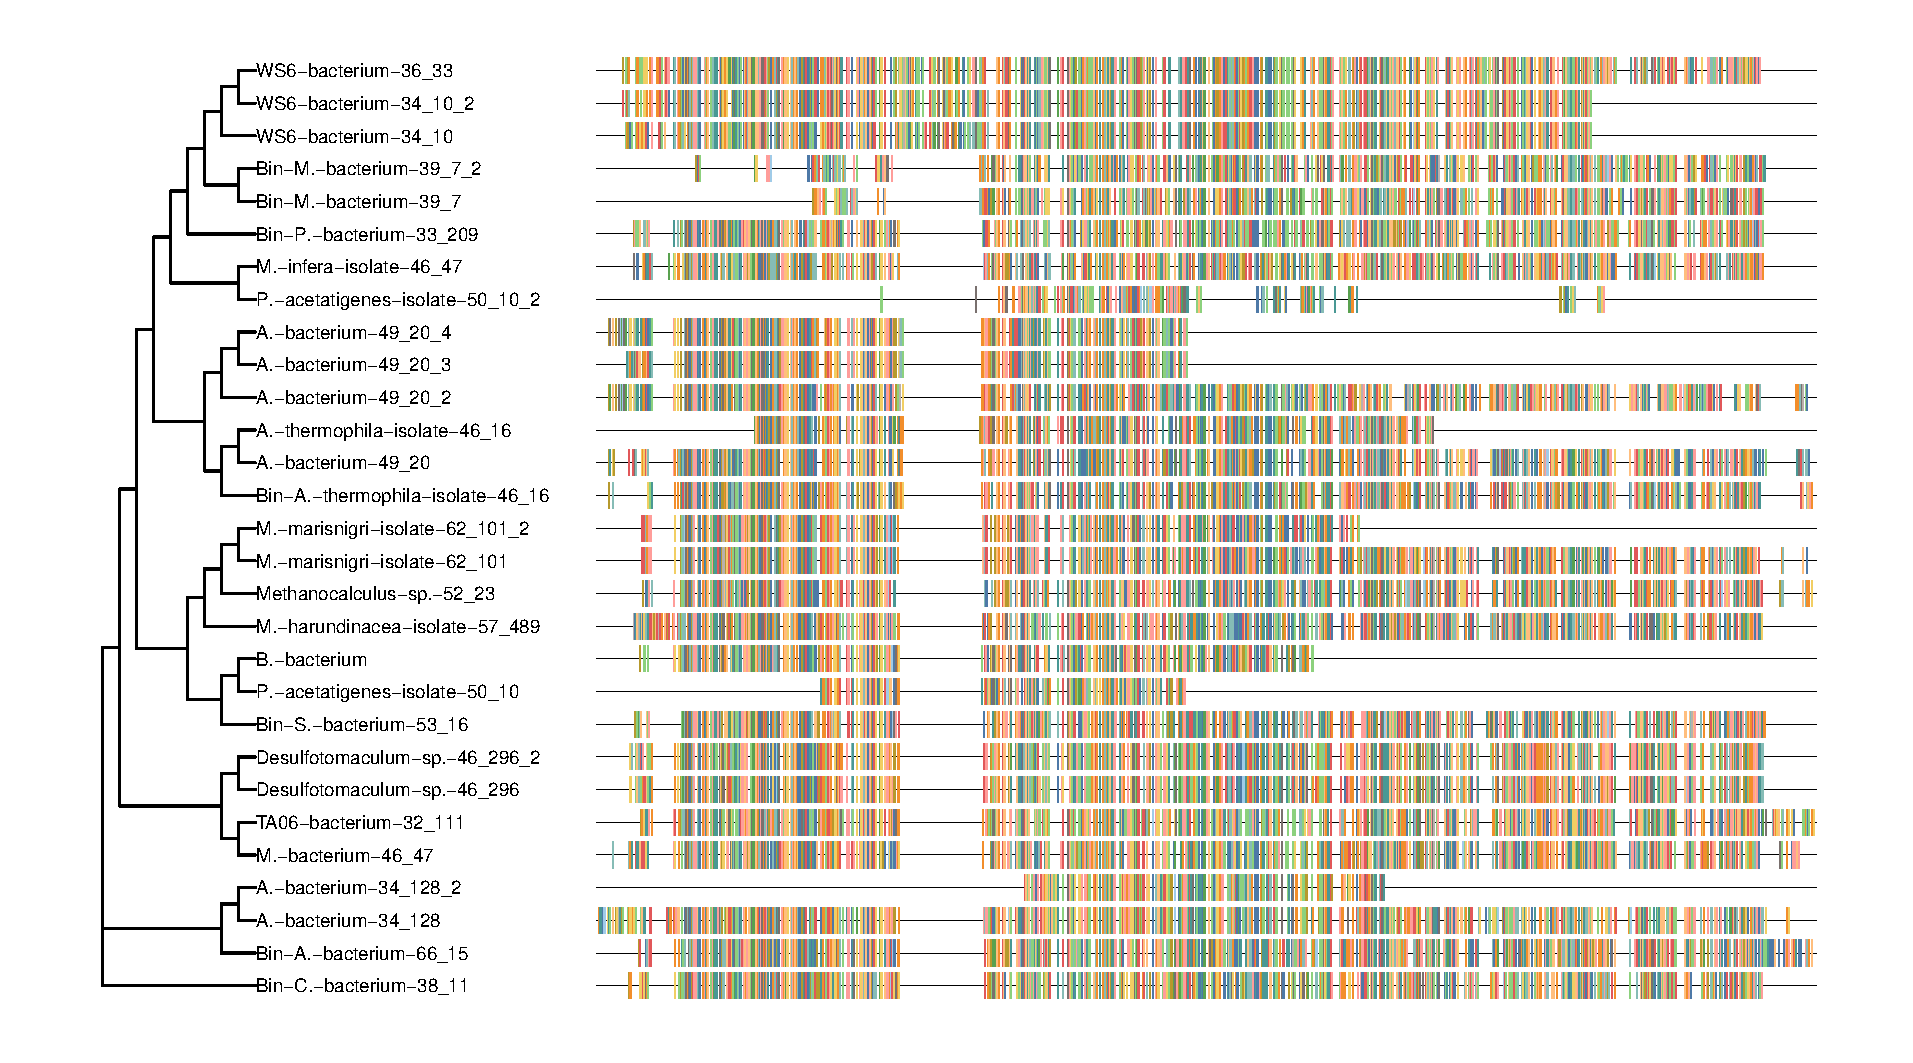
\includegraphics[width=\linewidth]{figures/gyrA-cdhit95-msa}
	\caption{A multiple sequence alignment and neighbor joining tree of representative gyrA amino acid fragments assembled by \plass from the genome neighborhoods in \hu. Protein sequences that originated from the genome bin are prepended with "Bin." All other sequences were assembled by Plass.
 }
 \label{fig:gyrAalign}
\end{figure*}

\subsection{gyrA by neighborhood}
\label{subsec:gyrAnbhd}

See Table~\ref{tab:gyrAcounts}. As can be seen in the left panel of figure 4 in the 
main text, we observe many unique amino acid sequences per single copy ortholog 
per query neighborhood.
Although we observe many possible traversal paths in compact De Bruijn graphs built
from reads that give rise to these sequences, we have no way to ascertain whether we
observed combinatorial complexity by assembling variants that would never be linked 
in nature. Therefore, we sought to conservatively estimate the number of positions
per amino acid sequence that contained variants using MAFFT alignments. First, we 
subsetted the alignment to sequences from one query neighborhood. Then we identified
all aligned non-gap characters for each position in the alignment (gaps were induced
in some neighborhoods by the presence of amino acid residues in other query neighborhood
amino acid sequences). For each of these positions, we counted the number of unique 
amino acid sequences per position, and the number of times each occurred at that position. 
We then elimated any variant that occurred fewer than 10 times. Lastly, we counted the 
number of well-supported distinct characters. We did this for gyrA, as well as the 
amino acid sequences for the other genes we tested (see other genes). Table~\ref{tab:gyrAcounts}
shows that we see increased number of gyrA sequences in many neighborhoods even with
this conservative approach.  

\subsection{Other genes}

\label{subsec:othergenes}

See bin and neighborhood content results for alaS in Table~\ref{tab:alaS}, gyrB in 
Table~\ref{tab:gyrB}, recA in Table~\ref{tab:recA}, rpb2d6 in Table~\ref{tab:rpb2d6}, 
rplB in Table~\ref{tab:rplB}, and rpsC in Table~\ref{tab:rpsC}. We selected gyrB and
recA because they were used by \hu to assign taxonomy to binned genomes. We selected
other genes used as single copy orthologs by programs like CheckM, and with longer PFAM
domains. 


\begin{table}
  \begin{tabular}{l l c c }
    \toprule
    Name & PFAM accession \\
    \midrule
    recA & PF00154 \\
    rplB & PF00181 \\
    rpsC & PF00189 \\
    gyrB & PF00204 \\
    gyrA & PF00521 \\
    rpb2d6 & PF00562 \\
    alaS & PF01411 \\
    \hline
    \bottomrule
  \end{tabular}
  \caption{Protein names and PFAM accessions for targeted analyses.}
  \label{tab:pfam_accessions}
\end{table}

\begin{table}
  \begin{tabular}{l l c c }
    \toprule
    Species & alaS (bin) & alaS (\plass) \\
    \midrule
    % generated from notebook 'tables/plass-genes/distinct_positions.ipynb'
    P. acetatigenes isolate 50\_10 & 0 & 0 \\
A. bacterium 49\_20 & 0 & 0 \\
P. bacterium 34\_609 & 0 & 0 \\
B. bacterium & 0 & 0 \\
S. bacterium 53\_16 & 0 & 0 \\
A. bacterium 34\_128 & 0 & 0 \\
M. infera isolate 46\_47 & 0 & 2 \\
M. marisnigri isolate 62\_101 & 0 & 2 \\
M. bacterium 39\_7 & 1 & 0 \\
Methanobacterium sp. 42\_16 & 1 & 1 \\
C. bacterium 38\_11 & 1 & 1 \\
S. bacterium 57\_84 & 1 & 1 \\
TA06 bacterium 32\_111 & 1 & 1 \\
P. bacterium 33\_209 & 1 & 1 \\
A. bacterium 66\_15 & 1 & 1 \\
M. harundinacea isolate 57\_489 & 1 & 1 \\
Methanocalculus sp. 52\_23 & 1 & 2 \\
WS6 bacterium 36\_33 & 1 & 2 \\
Desulfotomaculum sp. 46\_80 & 1 & 2 \\
M. bacterium 46\_47 & 1 & 2 \\
Desulfotomaculum sp. 46\_296 & 1 & 2 \\
A. thermophila isolate 46\_16 & 2 & 1 \\
WS6 bacterium 34\_10 & 2 & 2 \\

    \bottomrule
  \end{tabular}
  \caption{Bin and neighborhood alaS protein content.}
  \label{tab:alaS}
\end{table}

\begin{table}
  \begin{tabular}{l l c c }
    \toprule
    Species & gyrB (bin) & gyrB (\plass) \\
    \midrule
    % generated from notebook 'tables/plass-genes/distinct_positions.ipynb'
    M. bacterium 39\_7 & 0 & 0 \\
P. acetatigenes isolate 50\_10 & 0 & 0 \\
Methanobacterium sp. 42\_16 & 0 & 0 \\
WS6 bacterium 36\_33 & 0 & 0 \\
P. bacterium 34\_609 & 0 & 0 \\
Desulfotomaculum sp. 46\_80 & 0 & 0 \\
S. bacterium 57\_84 & 0 & 0 \\
S. bacterium 53\_16 & 0 & 0 \\
A. thermophila isolate 46\_16 & 0 & 2 \\
P. bacterium 33\_209 & 1 & 0 \\
C. bacterium 38\_11 & 1 & 1 \\
M. infera isolate 46\_47 & 1 & 1 \\
M. bacterium 46\_47 & 1 & 1 \\
TA06 bacterium 32\_111 & 1 & 1 \\
A. bacterium 66\_15 & 1 & 1 \\
M. harundinacea isolate 57\_489 & 1 & 1 \\
WS6 bacterium 34\_10 & 1 & 2 \\
Methanocalculus sp. 52\_23 & 1 & 2 \\
M. marisnigri isolate 62\_101 & 1 & 2 \\
A. bacterium 34\_128 & 1 & 2 \\
A. bacterium 49\_20 & 2 & 2 \\
B. bacterium & 2 & 2 \\
Desulfotomaculum sp. 46\_296 & 2 & 2 \\

    \bottomrule
  \end{tabular}
  \caption{Bin and neighborhood gyrB protein content.}
  \label{tab:gyrB}
\end{table}

\begin{table}
  \begin{tabular}{l l c c }
    \toprule
    Species & recA (bin) & recA (\plass) \\
    \midrule
    % generated from notebook 'tables/plass-genes/distinct_positions.ipynb'
    M. bacterium 39\_7 & 0 & 0 \\
WS6 bacterium 34\_10 & 0 & 0 \\
Methanocalculus sp. 52\_23 & 0 & 0 \\
A. bacterium 49\_20 & 0 & 0 \\
WS6 bacterium 36\_33 & 0 & 0 \\
P. bacterium 34\_609 & 0 & 0 \\
M. marisnigri isolate 62\_101 & 0 & 0 \\
S. bacterium 53\_16 & 0 & 0 \\
M. bacterium 46\_47 & 0 & 0 \\
A. thermophila isolate 46\_16 & 0 & 1 \\
B. bacterium & 1 & 0 \\
P. acetatigenes isolate 50\_10 & 1 & 1 \\
Methanobacterium sp. 42\_16 & 1 & 1 \\
C. bacterium 38\_11 & 1 & 1 \\
M. infera isolate 46\_47 & 1 & 1 \\
S. bacterium 57\_84 & 1 & 1 \\
A. bacterium 34\_128 & 1 & 1 \\
TA06 bacterium 32\_111 & 1 & 1 \\
P. bacterium 33\_209 & 1 & 1 \\
A. bacterium 66\_15 & 1 & 1 \\
M. harundinacea isolate 57\_489 & 1 & 1 \\
Desulfotomaculum sp. 46\_80 & 1 & 2 \\
Desulfotomaculum sp. 46\_296 & 1 & 2 \\

    \bottomrule
  \end{tabular}
  \caption{Bin and neighborhood recA protein content.}
  \label{tab:recA}
\end{table}

\begin{table}
  \begin{tabular}{l l c c }
    \toprule
    Species & rpb2d6 (bin) & rpb2d6 (\plass) \\
    \midrule
    % generated from notebook 'tables/plass-genes/distinct_positions.ipynb'
    P. acetatigenes isolate 50\_10 & 0 & 0 \\
P. bacterium 34\_609 & 0 & 0 \\
S. bacterium 57\_84 & 0 & 1 \\
M. bacterium 46\_47 & 0 & 1 \\
C. bacterium 38\_11 & 1 & 0 \\
A. bacterium 49\_20 & 1 & 0 \\
M. bacterium 39\_7 & 1 & 1 \\
Methanobacterium sp. 42\_16 & 1 & 1 \\
Methanocalculus sp. 52\_23 & 1 & 1 \\
M. infera isolate 46\_47 & 1 & 1 \\
B. bacterium & 1 & 1 \\
S. bacterium 53\_16 & 1 & 1 \\
A. bacterium 34\_128 & 1 & 1 \\
TA06 bacterium 32\_111 & 1 & 1 \\
A. bacterium 66\_15 & 1 & 1 \\
A. thermophila isolate 46\_16 & 1 & 1 \\
WS6 bacterium 36\_33 & 1 & 2 \\
Desulfotomaculum sp. 46\_80 & 1 & 2 \\
M. marisnigri isolate 62\_101 & 1 & 2 \\
Desulfotomaculum sp. 46\_296 & 1 & 2 \\
P. bacterium 33\_209 & 1 & 2 \\
M. harundinacea isolate 57\_489 & 1 & 2 \\
WS6 bacterium 34\_10 & 2 & 2 \\

    \bottomrule
  \end{tabular}
  \caption{Bin and neighborhood rpb2d6 protein content.}
  \label{tab:rpb2d6}
\end{table}

\begin{table}
  \begin{tabular}{l l c c }
    \toprule
    Species & rplB (bin) & rplB (\plass) \\
    \midrule
    % generated from notebook 'tables/plass-genes/distinct_positions.ipynb'
    M. bacterium 39\_7 & 0 & 0 \\
Methanobacterium sp. 42\_16 & 0 & 0 \\
Methanocalculus sp. 52\_23 & 0 & 0 \\
WS6 bacterium 36\_33 & 0 & 0 \\
M. marisnigri isolate 62\_101 & 0 & 0 \\
M. harundinacea isolate 57\_489 & 0 & 0 \\
P. acetatigenes isolate 50\_10 & 1 & 1 \\
C. bacterium 38\_11 & 1 & 1 \\
A. bacterium 49\_20 & 1 & 1 \\
M. infera isolate 46\_47 & 1 & 1 \\
P. bacterium 34\_609 & 1 & 1 \\
Desulfotomaculum sp. 46\_80 & 1 & 1 \\
S. bacterium 57\_84 & 1 & 1 \\
B. bacterium & 1 & 1 \\
S. bacterium 53\_16 & 1 & 1 \\
A. bacterium 34\_128 & 1 & 1 \\
M. bacterium 46\_47 & 1 & 1 \\
Desulfotomaculum sp. 46\_296 & 1 & 1 \\
TA06 bacterium 32\_111 & 1 & 1 \\
P. bacterium 33\_209 & 1 & 1 \\
A. bacterium 66\_15 & 1 & 1 \\
A. thermophila isolate 46\_16 & 1 & 1 \\
WS6 bacterium 34\_10 & 1 & 2 \\

    \bottomrule
  \end{tabular}
  \caption{Bin and neighborhood rplB protein content.}
  \label{tab:rplB}
\end{table}

\begin{table}
  \begin{tabular}{l l c c }
    \toprule
    Species & rpsC (bin) & rpsC (\plass) \\
    \midrule
    % generated from notebook 'tables/plass-genes/distinct_positions.ipynb'
    M. bacterium 39\_7 & 0 & 0 \\
P. acetatigenes isolate 50\_10 & 0 & 0 \\
WS6 bacterium 34\_10 & 0 & 0 \\
Methanobacterium sp. 42\_16 & 0 & 0 \\
Methanocalculus sp. 52\_23 & 0 & 0 \\
WS6 bacterium 36\_33 & 0 & 0 \\
M. marisnigri isolate 62\_101 & 0 & 0 \\
B. bacterium & 0 & 0 \\
P. bacterium 33\_209 & 0 & 0 \\
M. harundinacea isolate 57\_489 & 0 & 0 \\
M. infera isolate 46\_47 & 0 & 1 \\
C. bacterium 38\_11 & 1 & 1 \\
A. bacterium 49\_20 & 1 & 1 \\
P. bacterium 34\_609 & 1 & 1 \\
S. bacterium 57\_84 & 1 & 1 \\
S. bacterium 53\_16 & 1 & 1 \\
A. bacterium 34\_128 & 1 & 1 \\
M. bacterium 46\_47 & 1 & 1 \\
TA06 bacterium 32\_111 & 1 & 1 \\
A. bacterium 66\_15 & 1 & 1 \\
A. thermophila isolate 46\_16 & 1 & 1 \\
Desulfotomaculum sp. 46\_80 & 1 & 2 \\
Desulfotomaculum sp. 46\_296 & 1 & 2 \\

    \bottomrule
  \end{tabular}
  \caption{Bin and neighborhood rpsC protein content.}
  \label{tab:rpsC}
\end{table}
